% ------------------------------------------------------------------------------------------------
% Chirag's second subsection for Section 4: a check and repair of Model 3 (the pre-date network).
% Models 1-3 and their text are unchanged; this subsection only adds an audit and a repaired variant.
% Needs: booktabs, graphicx, figures/fig_model3.pdf and the entries in perceptions.bib.
% Every number is generated by code/model3_fix/ (summarize.py -> numbers.json).
% ------------------------------------------------------------------------------------------------
\subsection{Repairing the pre-date model (Model 3)}\label{sec:model3fix}

Model 3 asks how well a match can be predicted from what is known before the date. Re-running the
committed script (\texttt{pc-mle/pc\_mle\_analysis.py}) on the committed data reproduces its
held-out AUC of <<orig_their_auc>> and F1 of <<orig_their_f1>> exactly. Reading the code, we found
four problems.

\paragraph{What goes wrong.} \emph{(i) A post-date rating leaks in.} The script's list of
post-date columns contains \texttt{sinsere\_o}, but the column is spelled \texttt{sincere\_o}: the partner's
rating of the participant's sincerity, made on the scorecard after the date. It ranks
<<sincere_rank>> by mutual information and becomes a parent of \texttt{match}. Without it the
pipeline gives AUC <<noleak_their_auc>> and F1 <<noleak_their_f1>>, exactly the numbers in the
repository's README (once one learned edge is dropped; see (iv)). \emph{(ii) The table for \texttt{match} cannot be estimated.} The five
top-ranked variables are forced to be parents of \texttt{match}. Two of them have many states:
\texttt{field} is free text with <<field_values>> values, and
\texttt{expected\_num\_interested\_in\_me} (<<enii_missing>> missing) becomes a 19-state category.
Mutual information favours many-valued variables: with the labels shuffled, \texttt{field} still
gets <<field_null>> of its <<field_mi>> millinats, more than any other variable gets with the real
labels. The
CPT of \texttt{match} has <<orig_configs>> parent configurations for <<n_train>> training rows, so
maximum likelihood gives <<orig_frac01>> of the test rows a probability of exactly 0 or 1 (yet
<<p0_obs>> of the rows given probability 0 did match), and the log loss is <<orig_their_ll>> against
<<const_their_ll>> for always predicting the base rate.
\emph{(iii) The split rewards recognising people.} With a random row split, every test participant
also appears in training, and <<mirror>> of test rows have their mirrored row (the same date seen
from the other side, with the same \texttt{match} label) in training. For <<orig_seen>> of test
rows, the exact parent configuration of \texttt{match} occurred in training, and for <<lookup_only>>
it occurred only in rows of the same participant, so the CPT works as a lookup table of people. On events the model never saw (5 folds grouped by wave, so no person and no
date is on both sides), the committed pipeline scores AUC <<orig_wave_auc>>
(95\% interval <<orig_wave_ci>>, resampling waves). \emph{(iv) The run is fragile.}<<fragile>>

\paragraph{The repair.} Table~\ref{tab:model3} applies the fixes one at a time. Fixes 1--4 remove
the leak, recode \texttt{field} into its 18 coded categories, drop the <<enii_missing>>-missing column and the
wave identifier, keep \texttt{d\_age} (the only genuine pre-date difference), correct mutual
information for the number of states, let PC choose the family of \texttt{match}, and smooth with
a BDeu prior. Even then the network stays at chance on new events (AUC <<bdeu_wave_auc>>, log loss
<<bdeu_wave_ll>>, worse than the base rate). PC links \texttt{match} to <<pc_kids_range>>
variables, and which ones changes from fold to fold, so these dependencies do not carry over to
other events. Fix 5 keeps the same ten variables and the same estimator, but fixes the structure
instead of learning it: \texttt{match} is a parent of every variable (naive Bayes). This gives AUC
<<nb_wave_auc>> on new events (95\% interval <<nb_wave_ci>>; between <<nb_fold_min>> and
<<nb_fold_max>> in every fold), with a log loss slightly below the base rate's. A logistic regression on all
<<n_lr_vars>> pre-date variables does no better (<<lr_wave_auc>>). A tree-augmented naive Bayes
\cite{friedman1997bayesian} does slightly worse (<<tan_wave_auc>>), and adding PC's edges on top of
naive Bayes does much worse (<<pcnb_wave_auc>>). The variables chosen in all five folds are the
participant's expected number of matches, how much both people value shared interests, and two
hobbies (<<nb_always>>).

\begin{table}[t]
\centering\small
\caption{Model 3 after each fix, cumulatively. AUC and log loss for \texttt{match} on the team's
85/15 row split (<<n_test>> test rows) and on new events (5 folds grouped by wave, all
<<n_rows>> rows). Always predicting the base rate gives log loss <<const_their_ll>> and
<<const_wave_ll>>.}\label{tab:model3}
\begin{tabular}{@{}lcccc@{}}
\toprule
& \multicolumn{2}{c}{Row split} & \multicolumn{2}{c}{New events}\\
\cmidrule(lr){2-3}\cmidrule(l){4-5}
Model & AUC & Log loss & AUC & Log loss\\
\midrule
As committed: PC, 5 forced parents, MLE & <<orig_their_auc>> & <<orig_their_ll3>> & <<orig_wave_auc>> & <<orig_wave_ll>>\\
1\quad drop the leaked \texttt{sincere\_o} & <<noleak_their_auc>> & <<noleak_their_ll>> & <<noleak_wave_auc>> & <<noleak_wave_ll>>\\
2\quad + recode, drop, correct MI & <<recode_their_auc>> & <<recode_their_ll>> & <<recode_wave_auc>> & <<recode_wave_ll>>\\
3\quad + PC chooses the family of \texttt{match} & <<pcpar_their_auc>> & <<pcpar_their_ll>> & <<pcpar_wave_auc>> & <<pcpar_wave_ll>>\\
4\quad + BDeu prior (ESS 5) & <<bdeu_their_auc>> & <<bdeu_their_ll>> & <<bdeu_wave_auc>> & <<bdeu_wave_ll>>\\
5\quad + \texttt{match} $\to$ every variable (repaired) & \textbf{<<nb_their_auc>>} & \textbf{<<nb_their_ll>>} & \textbf{<<nb_wave_auc>>} & \textbf{<<nb_wave_ll>>}\\
\midrule
Tree-augmented naive Bayes & <<tan_their_auc>> & <<tan_their_ll>> & <<tan_wave_auc>> & <<tan_wave_ll>>\\
PC edges + \texttt{match} $\to$ every variable & <<pcnb_their_auc>> & <<pcnb_their_ll>> & <<pcnb_wave_auc>> & <<pcnb_wave_ll>>\\
Logistic regression, all pre-date variables & <<lr_their_auc>> & <<lr_their_ll>> & <<lr_wave_auc>> & <<lr_wave_ll>>\\
\bottomrule
\end{tabular}
\end{table}

\begin{figure}[t]
\centering
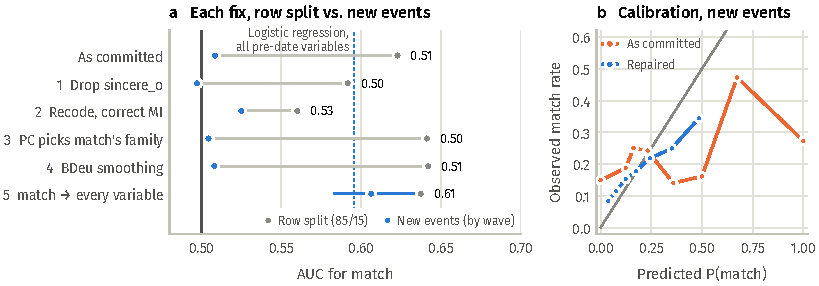
\includegraphics[width=\linewidth]{figures/fig_model3.pdf}
\caption{(a) AUC after each fix on the row split (grey) and on new events (blue; bar: 95\%
interval resampling waves). The row split flatters every version; only the repaired structure
holds up on new events. (b) On new events, <<wave_p05>> of the committed network's
predictions are exactly 0.5 (a parent configuration never seen in training), and its predictions of
exactly 0 and 1 come true <<wave_p0_obs>> and <<wave_p1_obs>> of the time; the repaired network's
probabilities follow the diagonal.}\label{fig:model3}
\end{figure}

\paragraph{What this means.} Prospective prediction is possible but weak: about 0.6 AUC on new
people, compared with the much stronger signal in the post-date ratings
(Section~\ref{sec:perceptions}). The committed pipeline's row-split score of
<<orig_their_auc_short>> is close to the repaired model's <<nb_their_auc_short>>, but for the wrong
reasons: on new events it falls to <<orig_wave_auc_short>>, while the repaired model keeps
<<nb_wave_auc_short>> (difference <<nb_minus_orig>>, 95\% interval <<nb_minus_orig_ci>>). Learning
the class variable's family by independence tests is fragile when every link to it is weak, and a
row split cannot reveal this. Details are in Appendix~\ref{app:model3fix}.
